\section {Nanomaterials and Nanostructures}
A nanostructure is defined as a material system or object, where
at least one of the dimensions lies below 100 nm. Nanostructures
can be classified into three different categories:
\begin{enumerate}
\item zero-dimensional (0D)
\item one-dimensional (1D)
\item two-dimensional (2D)
\end{enumerate}
0D nanostructures are materials in which all three dimensions are at the nanoscale. A good example of these materials are buckminster fullerenes  and quantum dots. 1D nanostructures are materials that have two physical dimensions in the nanometer range, while the third dimension can be large, such as in the carbon nanotube. 2D nanostructures, or thin films, only have one dimension in the nanometer range and are used readily in the processing of complimentary metal-oxide semiconductor transistors and micro-electro-mechanical systems (MEMS). Nanomaterials are the base material of many nanoscale objects. Recently various one-dimensional nanostructures have been realized. They include nanodots, nanorods, nanowires, nanobelts, nanotubes, nanobridges and nanonails, nanowalls, nanohelices, seamless nanorings. Among all the one-dimensional nanostructures, nanotubes, nanorods and nanowires are widely studied. This is because of the easy material formation and device applications.

Nanostructures have unique properties when compared to their individual atoms or
molecules or their bulk macroscopic properties. For example, bulk material such as
Copper wire, their intrinsic properties, say density or conductivity, are independent
of its size. That is, if a 1 m long Copper wire, when cut into few pieces, and for these pieces, if the density or conductivity is measured, one will find they are same as the original Copper wire. If the dividing process is done indefinitely, then the property invariance will still remain. However, if the division is made at the electron, proton or neutron levels, that is at the nanoscale levels, we can certainly expect significant change in the property of the nanostructures. The properties of the nanoscale material systems can get significantly affected by the following three phenomenon:
\begin{itemize}
\item \textit{Quantum Confinement}: The confinement of electrons in the nanoscale dimensions will result in the change in the energy and momentum of the nano material system, which in turn significantly alters its properties.
\item \textit{Quantum Coherence}: : This phenomenon relates to the phase relation of the wave function in nano material system, that is preserved in the nanomaterial system. The quantum coherence property is well maintained in atoms and molecules but not always in nanostructures due to inherent defects present in these structures.
This results in the change of properties in the nano scale and hence it is necessary
to consider both the quantum coherence and de-coherence effects while dealing
with nanostructures.
\item \textit{Surface Effects}: Vast majority of the atoms in a nanostructures are located either at the surfaces or interfaces. The properties of these surface atoms can be quite different than that of those, which are located in the interior.
\end{itemize}

The above factors significantly alter the properties of the nanostructures as compared to their bulk material. For a nanomaterial systems, both the crystalline state and surface/interface state is very important. These materials are often in metastable state. Their atomic configuration depends on the kinetic process in which they are fabricated or grown. Therefore, the properties of nanostructures can be adjusted or manipulated by changing its size, shape or the process by which it is made, which can often lead to some rich and surprising outcomes.

\section {Carbon Nanotubes}
Carbon is a remarkable element that has a unique structures which make it amenable
to combine with other elements and compounds to get a new compound. It is said
that carbon has the ability for form close to 10 million different compounds. It is
present in the food we eat, the clothes we wear, the cosmetics we use and also in
the fuel that drives our cars. Carbon exists in four different allotropes, namely the
amorphous, the graphite, the diamond and the fullerene. The Amorphous carbon
structure is visually a highly disordered structure. It is for this reason that it lacks
structural integrity . This carbon structure forms at the edges or is the residue of other
elemental compounds. The disorder of this structure allows it to have many available
bonds and is responsible for building more complex carbon based molecules.

There are many definitions to nanotubes. The simplest definition of nanotube is that
it is a nanometer scale structure that resembles a tube. There are both organic and
inorganic nanotubes. Organic nanotubes are the carbon nanotubes or CNT. With
respect to Carbon NanoTube (CNT), a nanotube can be defined as \emph{a long cylindrical carbon structure
consisting of hexagonal graphite molecules attached at the edges}. Some nanotubes
have a single cylinder while others have two or more concentric cylinders. Nanotubes
have several characteristics, namely wall thickness, number of concentric cylinders,
cylinder radius, and cylinder length. Some nanotubes have a property called chirality,
an expression of longitudinal twisting.

\subsection {Types and structures}
Carbon nanotubes are basically sheets of graphite rolled up into a tube as shown in this figure. Hence, the hexagonal two dimensional lattice of graphite is mapped on a one-dimensional cylinder of radius R with various helicities characterized by the rolling vectors (n,m).\cite{types_taner} Nanotubes form different types, which can be described by the chiral vector $(n, m)$, where $n\text{ and }m$ are integers of the vector equation $R = n a_1 + m a_2$. The chiral vector is determined by the diagram at the left. Imagine that the nanotube is unraveled into a planar sheet. Draw two lines (the blue lines) along the tube axis where the separation takes place. In other words, if you cut along the two blue lines and then match their ends together in a cylinder, you get the nanotube that you started with. Now, find any point on one of the blue lines that intersects one of the carbon atoms (point A). Next, draw the Armchair line (the thin yellow line), which travels across each hexagon, separating them into two equal halves. Now that you have the armchair line drawn, find a point along the other tube axis that intersects a carbon atom nearest to the Armchair line (point B). Now connect A and B with our chiral vector, $R$ (red arrow). The wrapping angle $\phi$; (not shown) is formed between $R$ and the Armchair line. If $R$ lies along the Armchair line ($\phi=0^\circ$), then it is called an "\textit{Armchair}" nanotube. If $\phi=30^\circ$, then the tube is of the "\textit{zigzag}" type. Otherwise, if $\phi \ll 30^\circ$ then it is a "\textit{chiral}" tube. The vector $a_1$ lies along the "\textit{zigzag}" line. The other vector $a_2$ has a different magnitude than $a_1$, but its direction is a reflection of $a_1$ over the Armchair line. When added together, they equal the chiral vector $R$.
The values of $n\text{ and }m$ determine the chirality, or "twist" of the nanotube. The chirality in turn affects the conductance of the nanotube, it's density, it's lattice structure, and other properties. A SWNT is considered metallic if the value $n - m$ is divisible by three. Otherwise, the nanotube is semiconducting. Consequently, when tubes are formed with random values of n and m, we would expect that two-thirds of nanotubes would be semi-conducting, while the other third would be metallic, which happens to be the case.\cite{eqstruct}
Given the chiral vector (n,m), the diameter of a carbon nanotube can be determined using the relationship\\
\[d = (n^2 + m^2 + nm)^{1/2} \times 0.0783 nm\]
\begin{figure}
\centering
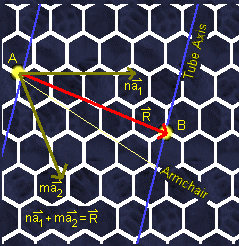
\includegraphics[scale=1]{typesNT.png}
\caption{Illustration of rolling vectors (n,m)}
\label{typesNT}
\end{figure}
\begin{figure}
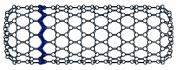
\includegraphics[scale=1]{n0tube.jpg}
\caption{(n,0) zigzag nanotube }
\label{n0tube}
\end{figure}
\begin{figure}
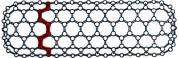
\includegraphics[scale=1]{nntube.jpg}
\caption{(n,n) armchair nanotube}
\label{nntube}
\end{figure}
\begin{figure}
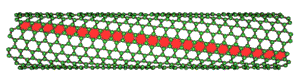
\includegraphics[scale=1]{nmtube.png}
\caption{(n,m) chiral nanotube}
\label{nmtube}
\end{figure}
\subsection {Why study Carbon nanotubes?}
Carbon nanotubes are molecular-scale tubes of graphitic carbon with outstanding properties. They are among the stiffest and strongest fibres known, and have remarkable electronic properties and many other unique characteristics. For these reasons they have attracted huge academic and industrial interest, with thousands of papers on nanotubes being published every year. Commercial applications have been rather slow to develop, however, primarily because of the high production costs of the best quality nanotubes.

The current huge interest in carbon nanotubes is a direct consequence of the synthesis of buckminsterfullerene, $C_{60}$, and other fullerenes, in 1985. The discovery that carbon could form stable, ordered structures other than graphite and diamond stimulated researchers worldwide to search for other new forms of carbon. The search was given new impetus when it was shown in 1990 that $C_{60}$ could be produced in a simple arc-evaporation apparatus readily available in all laboratories. It was using such an evaporator that the Japanese scientist Sumio Iijima discovered fullerene-related carbon nanotubes in 1991\cite{iijima1991helical}. The tubes contained at least two layers, often many more, and ranged in outer diameter from about 3 nm to 30 nm. They were invariably closed at both ends.

The strength of the $\mathrm{sp^2}$ carbon-carbon bonds gives carbon nanotubes amazing mechanical properties. The stiffness of a material is measured in terms of its Young's modulus, the rate of change of stress with applied strain. The Young's modulus of the best nanotubes can be as high as 1000 GPa which is approximately 5x higher than steel. The tensile strength, or breaking strain of nanotubes can be up to 63 GPa, around 50x higher than steel. These properties, coupled with the lightness of carbon nanotubes, gives them great potential in applications such as aerospace. It has even been suggested that nanotubes could be used in the “space elevator”, an Earth-to-space cable first proposed by Arthur C. Clarke. The electronic properties of carbon nanotubes are also extraordinary. Especially notable is the fact that nanotubes can be metallic or semiconducting depending on their structure. Thus, some nanotubes have conductivities higher than that of copper, while others behave more like silicon. There is great interest in the possibility of constructing nanoscale electronic devices from nanotubes, and some progress is being made in this area. However, in order to construct a useful device we would need to arrange many thousands of nanotubes in a defined pattern, and we do not yet have the degree of control necessary to achieve this. There are several areas of technology where carbon nanotubes are already being used. These include flat-panel displays, scanning probe microscopes and sensing devices. The unique properties of carbon nanotubes will undoubtedly lead to many more applications.\cite{importance}
\subsection {Why study wave propagation in CNTs?}
Increasing emphasis of miniature devices have made the scientists to look for newer
and novel materials which can be handled at the atomistic scales. In this regard,
Nanoscale materials and structures with nano thicknesses have attracted consider-
able interest from the scientific community in the fields of microelectronics and
nanotechnology. More and more nanostructures, e.g. ultra-thin films, nanowires
and nanotubes, have been fabricated and served as the basic building blocks for
nano-electro-mechanical-systems (NEMS). For long-term stability and reliability of
various devices at nanoscale, researchers should possess a deep understanding and
knowledge of mechanical properties of nano-materials and -structures, especially the
time dependent or dynamic properties.

Nanostructures such as CNTs can propagate waves of the order of terahertz (THz). As dimensions of the material become smaller, however, their resistance to deformation is increasingly determined by internal or external discontinuities (such as surfaces, grain boundary, strain
gradient, and dislocation). Although many sophisticated approaches for predicting
the mechanical properties of nanomaterials have been reported, few addressed the
challenges posed by interior nanostructures such as the surfaces, interfaces, struc-
tural discontinuities and deformation gradient of the nanomaterials under extreme
loading conditions. The use of atomistic simulation may be a potential solution in
the long run. However, it is well known that the capability of this approach is much
limited by its need of prohibitive computing time and an astronomical amount of data
generated in the calculations. Wave propagation analysis using continuum models,
especially using non-local elasticity models can used to address the above problems.

Wave propagation studies mainly include the estimation of wavenumber and wave
speeds such as phase and group speeds. The concept of group velocity may be useful
in understanding the dynamics of carbon nanotubes, since it is related to the energy
transportation of wave propagation. It is useful to study the
wave propagation in nanostructures, so as to examine the effect of length scales on
the wave dispersion from the viewpoint of group velocity or energy transportation. To
describe the effect of microstructures of a nanostructures on its mechanical properties,
it is assumed that the model of the nanostructure is made of a kind of non-local elastic
material, where the stress state at a given reference location depends not only on the
strain of this location but also on the higher order gradient of strain, so as to take
the influence of the microstructures into account. It is reported that both local elastic
models (where effects of nano scale is not considered) and non-local elastic models
(where the effect of scale is considered) can offer the correct prediction when the
wavenumber is lower. However, the results of the elastic model remarkably deviate
from those given by the non-local elastic model with an increase in the wavenumber.
As a result, the microstructures play an important role in the dispersion of waves in
nanoscale structures. Since terahertz physics of nanoscale materials and devices are
the main concerns in wave characteristics of CNTs, the small-scale effect must be
of significance in achieving accurate dispersion relations as the wavelength in the
frequency domain is in the order of nanometers.\cite{gopalakrishnan2013wave}
